% !TEX program = xelatex
\documentclass[11pt,a4paper]{article}

\usepackage[margin=2.2cm]{geometry}
\usepackage{fontspec}
\usepackage{xeCJK}
\setCJKmainfont{Microsoft YaHei}[
  BoldFont=Microsoft YaHei Bold,
  AutoFakeBold=true
]
\setCJKsansfont{Microsoft YaHei}
\setmainfont{Times New Roman}
\setsansfont{Arial}
\setmonofont{Consolas}

\usepackage{amsmath,amssymb}
\usepackage{booktabs}
\usepackage{tabularx}
\usepackage{graphicx}
\usepackage{float}
\usepackage{caption}
\usepackage{subcaption}
\usepackage{hyperref}
\usepackage{xcolor}
\usepackage{enumitem}
\usepackage{listings}
\usepackage{multirow}
\usepackage{array}
\usepackage{siunitx}

\hypersetup{
  colorlinks=true,
  linkcolor=black!70,
  urlcolor=blue!50!black,
  citecolor=black!70
}

\captionsetup{font=small, labelfont=bf}
\graphicspath{{../outputs/figures/}}

\lstset{
  basicstyle=\ttfamily\small,
  breaklines=true,
  frame=single,
  backgroundcolor=\color{gray!8},
  columns=fullflexible
}

\title{\bfseries 基于图神经网络的芯片封装二维稳态热场代理模型\\[0.4em]
\large 技术说明文档（chip-thermal-gnn）}
\author{项目自动生成报告（实验结果均为本机实测）}
\date{\today}

\begin{document}
\maketitle
\tableofcontents
\newpage

% =========================================================
\section{项目概述}
% =========================================================

本项目实现了一个可复现的 Python 研究演示系统 \texttt{chip-thermal-gnn}，目标是构建
\textbf{基于图神经网络（GNN）的芯片封装二维稳态热场代理模型}，用于展示：
\begin{itemize}[leftmargin=1.5em]
  \item 有限元网格到图数据的转换与学习；
  \item 工程热仿真在多工况场景下的加速潜力；
  \item AI for Science（AI4S）在封装热分析中的落地路径。
\end{itemize}

项目\textbf{不依赖}任何企业内部代码、数据或模型；温度场标签全部由开源有限元库
\texttt{scikit-fem} 实际求解生成；报告中的全部数值指标均来自真实训练与测试运行，
\textbf{未伪造}。

\subsection{核心任务定义}
给定二维芯片封装截面的材料参数、热源工况与边界条件，代理模型直接预测网格各节点的
温升场
\[
\Delta T(\mathbf{x}) = T(\mathbf{x}) - T_{\mathrm{amb}},
\]
并与有限元真值对比，评估精度、泛化与推理速度。

\subsection{技术栈}
Python、PyTorch、PyTorch Geometric、NumPy、SciPy、scikit-fem、Matplotlib、Pandas、
PyYAML、pytest。

\subsection{项目目录结构}
\begin{lstlisting}
chip-thermal-gnn/
  README.md
  requirements.txt
  configs/          # 数据与训练配置
  data/raw/         # FEM 原始样本
  data/processed/   # PyG 图数据
  outputs/
    checkpoints/    # 最优权重
    figures/        # 可视化图片
    metrics/        # 指标表与评估摘要
  src/              # 全部可执行脚本
  tests/            # 单元测试
  docs/             # 本 LaTeX / PDF 文档
\end{lstlisting}


% =========================================================
\section{物理模型与假设}
% =========================================================

\subsection{几何结构}
采用二维矩形封装截面（宽 \(20\,\mathrm{mm}\)，高 \(12\,\mathrm{mm}\)），自下而上四层：
基板（Substrate）\(\to\) 铜散热层（Cu）\(\to\) 导热界面材料（TIM）\(\to\) Die（硅）。
几何示意与规则三角形有限元网格见图~\ref{fig:structure}。

\begin{figure}[H]
  \centering
  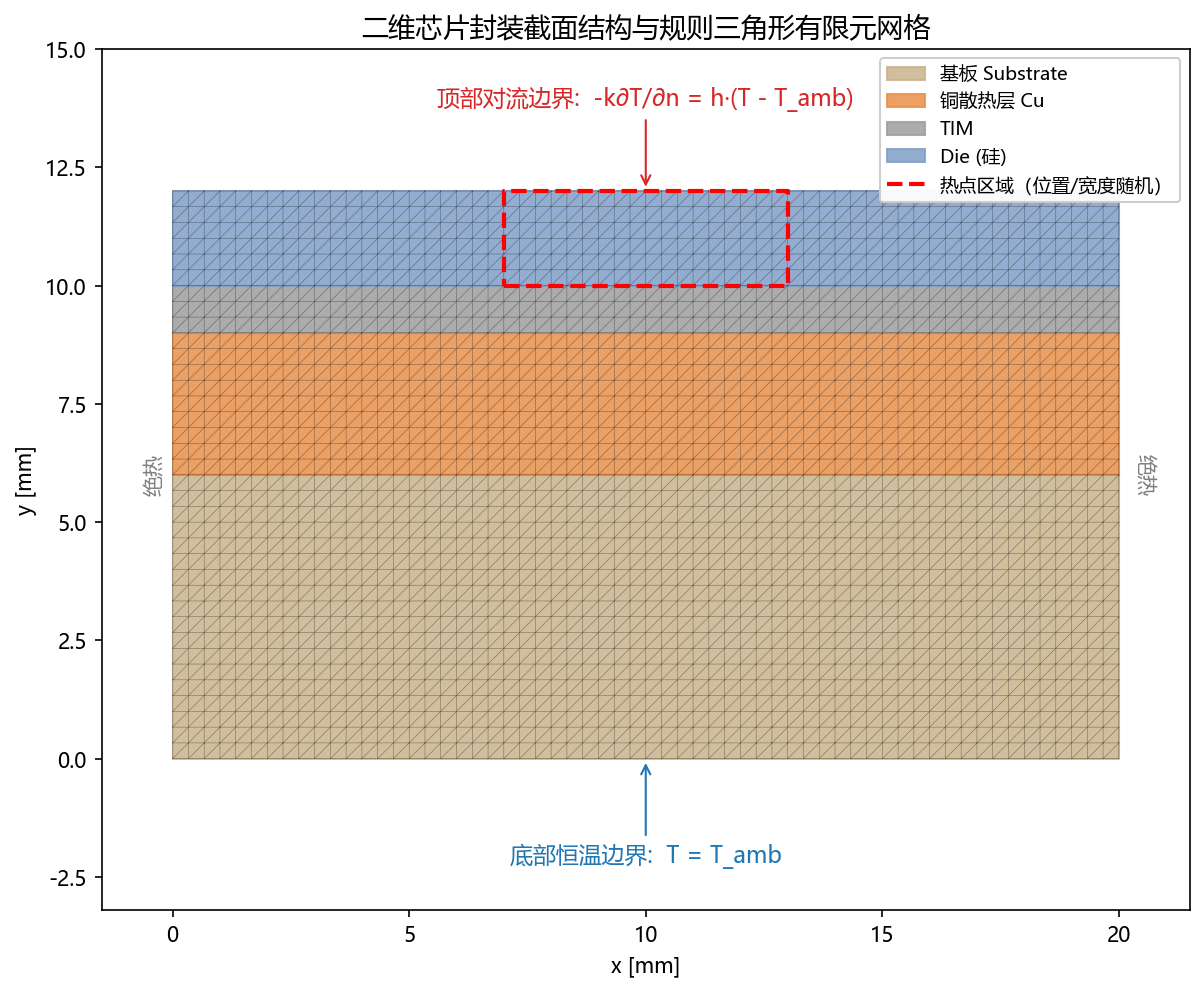
\includegraphics[width=0.95\textwidth]{package_structure_mesh.png}
  \caption{二维芯片封装截面结构与规则三角形有限元网格。顶部为对流边界，底部为恒温边界，
  左右绝热；红色虚线表示 Die 层中位置与宽度随机采样的热点区域。}
  \label{fig:structure}
\end{figure}

各层厚度与导热系数采样范围见表~\ref{tab:layers}。

\begin{table}[H]
\centering
\caption{封装层级、厚度与导热系数采样范围}
\label{tab:layers}
\begin{tabular}{llcc}
\toprule
层级 & 材料 & 厚度 & \(k\) 范围 [\si{W/(m\cdot K)}] \\
\midrule
基板 Substrate & 有机/陶瓷类 & \(6\,\mathrm{mm}\) & \(15\sim 60\) \\
散热层 & 铜 & \(3\,\mathrm{mm}\) & \(360\sim 400\) \\
界面材料 TIM & 膏体/垫片类 & \(1\,\mathrm{mm}\) & \(1\sim 8\)（OOD: \(0.2\sim 0.9\)） \\
Die & 硅 & \(2\,\mathrm{mm}\) & \(130\sim 155\) \\
\bottomrule
\end{tabular}
\end{table}

\subsection{控制方程}
稳态热传导：
\begin{equation}
-\nabla\cdot\big(k\nabla T\big)=q,
\label{eq:steady}
\end{equation}
其中 \(k(\mathbf{x})\) 为分材料导热系数，\(q(\mathbf{x})\) 为体热源功率密度。

\subsection{边界条件（简化设置）}
\begin{itemize}[leftmargin=1.5em]
  \item \textbf{顶部}（Die 上表面）：对流边界
  \[
  -k\frac{\partial T}{\partial n}=h_{\mathrm{top}}\big(T-T_{\mathrm{amb}}\big),
  \quad h_{\mathrm{top}}\in[500,15000]\,\mathrm{W/(m^2\cdot K)}
  \]
  （OOD 测试：\(100\sim 400\)）；
  \item \textbf{底部}（基板下表面）：恒温 Dirichlet 边界 \(T=T_{\mathrm{amb}}\)；
  \item \textbf{左右两侧}：绝热（零通量自然边界条件）。
\end{itemize}

\subsection{热源设置}
Die 层内施加体热源：背景功率密度 \(q_{\mathrm{base}}\in[10^5,5\times 10^5]\,\mathrm{W/m^3}\)
与矩形热点 \(q_{\mathrm{hot}}\in[5\times 10^6,3\times 10^7]\,\mathrm{W/m^3}\)
（OOD：\(3.5\times 10^7\sim 6\times 10^7\)）。热点中心位置与宽度在芯片宽度比例范围内随机采样。

\subsection{明确的物理简化假设}
\begin{enumerate}[leftmargin=1.5em]
  \item 二维截面近似（单位深度）；
  \item 各层厚度相对真实封装等比放大，便于规则网格质量与可视化；
  \item 材料线性、各向同性，\(k\) 与温度无关；
  \item 层间无额外接触热阻（TIM 层显式代表界面热阻）；
  \item 边界简化：底部理想恒温、侧面绝热、仅顶部对流；
  \item 关于 \(T_{\mathrm{amb}}\)：因问题线性且边界均以 \(T_{\mathrm{amb}}\) 为参考，
  温升场 \(\Delta T\) 在数学上与 \(T_{\mathrm{amb}}\) 取值无关；数据集中仍对其采样并保留特征，
  以便未来扩展到温度相关材料属性（非线性问题）。
\end{enumerate}


% =========================================================
\section{数据生成与图构建}
% =========================================================

\subsection{有限元离散}
使用 \texttt{scikit-fem} 的 \texttt{MeshTri.init\_tensor} 生成规则三角形网格：
\(61\times 37\) 节点，共 \textbf{2257} 个节点、\textbf{4320} 个三角单元。
所有样本共用同一张网格（固定几何、变工况）。单元采用线性三角元 \(P_1\)，
组装刚度矩阵与热源载荷，顶部叠加 Robin（对流）边界，底部施加 Dirichlet 条件后求解。

实测平均单次 FEM 求解耗时约 \(\mathbf{8.50\,\mathrm{ms}}\)（本机 RTX 3060 环境下的 SciPy
稀疏求解）。

\subsection{数据集划分}
共生成 \textbf{360} 个样本，划分见表~\ref{tab:split}。测试集中包含至少一种训练集未出现的
工况组合（更高热源功率、更差 TIM 导热系数、更差对流条件），用于验证外推泛化。

\begin{table}[H]
\centering
\caption{数据集划分}
\label{tab:split}
\begin{tabular}{lccc}
\toprule
子集 & 样本数 & 工况分布 & 说明 \\
\midrule
训练集 & 300 & 分布内 & 参数在配置范围内均匀采样 \\
验证集 & 30 & 分布内 & 早停与学习率调度 \\
测试集 & 30 & 20 分布内 + 10 OOD & OOD 含高功率/差 TIM/差对流 \\
\bottomrule
\end{tabular}
\end{table}

每个样本保存：节点坐标、材料类别、节点热源特征、边界特征、三角形连接关系、
节点温度场标签、工况元数据。原始数据位于 \texttt{data/raw/}，并写入包含采样范围、
划分与随机种子的 \texttt{metadata.json}（种子 \(=2024\)）。

\subsection{图数据表示}
每个 FEM 样本转换为一个 \texttt{torch\_geometric.data.Data} 对象，字段如下：

\begin{itemize}[leftmargin=1.5em]
  \item \(\mathbf{x}\in\mathbb{R}^{N\times 21}\)：节点特征。包含归一化坐标、材料 one-hot、
  局部热源强度、环境温度、边界换热系数与边界类型标志，以及\textbf{广播到全部节点的全局工况特征}
  （各层 \(k\)、\(q_{\mathrm{base}}/q_{\mathrm{hot}}\)、热点位置/宽度、TIM 与对流热阻）；
  \item \(\mathrm{edge\_index}\)：由三角单元生成的无向边（双向去重），共 \textbf{13152} 条有向边；
  \item \(\mathrm{edge\_attr}\in\mathbb{R}^{E\times 4}\)：归一化相对坐标 \((\Delta x,\Delta y)\)、
  边长、两端点导热系数的调和平均；
  \item \(\mathbf{y}\in\mathbb{R}^{N}\)：节点温升 \(\Delta T\)（优先预测温升而非绝对温度）；
  \item \(\mathrm{pos}\)：节点物理坐标，用于可视化。
\end{itemize}

\textbf{为何广播全局工况特征：}稳态导热是椭圆型方程，任一点温度受全域参数影响。
消息传递轮数有限（8 轮）而网格图直径约数十跳；若不广播，远离热源/边界的节点难以感知工况，
模型精度会受结构性限制。这是稳态（非时间步进）图代理模型的常见做法。


% =========================================================
\section{模型设计}
% =========================================================

\subsection{主模型：MeshGraphNet 风格 Encode--Process--Decode}
\begin{enumerate}[leftmargin=1.5em]
  \item \textbf{Node Encoder / Edge Encoder}：MLP 将节点/边特征映射到 128 维隐空间；
  \item \textbf{Processor}：8 轮残差消息传递。每轮先由源节点、目标节点与边隐变量经 MLP
  更新边隐变量（残差），再按目标节点求和聚合并经 MLP 更新节点隐变量（残差）；
  全部 MLP 带 LayerNorm 与 dropout；
  \item \textbf{Decoder}：两层 MLP 输出单节点标准化温升。
\end{enumerate}
主模型参数量约 \(\mathbf{979{,}329}\)。

实现参考 DeepMind MeshGraphNets（ICLR 2021）思想，代码从零编写；调研过的开源参考包括
DeepMind \texttt{meshgraphnets}（TensorFlow）与 NVIDIA PhysicsNeMo 的 PyTorch/PyG
\texttt{MeshGraphNet} 实现。公开预训练权重面向流体等其他场景，特征接口与本任务不兼容，
故在自建 FEM 数据上从零训练。

\subsection{基线模型}
4 层 GraphSAGE（可配置为 GCNConv），不使用边特征，直接回归节点温升；
参数量约 \(\mathbf{104{,}321}\)。

\subsection{损失函数与训练策略}
\begin{itemize}[leftmargin=1.5em]
  \item 主损失：在全局标准化温升空间中，采用\textbf{逐样本相对形式}
  （每样本误差能量除以该样本自身信号能量），避免高功率大温升样本主导损失；
  \item 辅助项：峰值温度误差（真实温升最大节点处的预测误差平方），权重 \(0.1\)；
  \item 优化器 Adam（\(\mathrm{lr}=10^{-3}\)），ReduceLROnPlateau，梯度裁剪，
  早停耐心 40，固定随机种子 2024，保存验证集最优权重。
\end{itemize}

训练实测摘要见表~\ref{tab:train}。

\begin{table}[H]
\centering
\caption{训练摘要（本机实测）}
\label{tab:train}
\begin{tabular}{lcccc}
\toprule
模型 & 最佳 epoch & 最佳验证损失 & 总训练轮数 & 训练时长 \\
\midrule
MeshGraphNet & 296 & 0.01404 & 336 & \(\approx 56\,\mathrm{min}\) \\
GraphSAGE 基线 & 265 & 0.00837 & 305 & \(\approx 4\,\mathrm{min}\) \\
\bottomrule
\end{tabular}
\end{table}

训练/验证损失曲线见图~\ref{fig:loss}。

\begin{figure}[H]
  \centering
  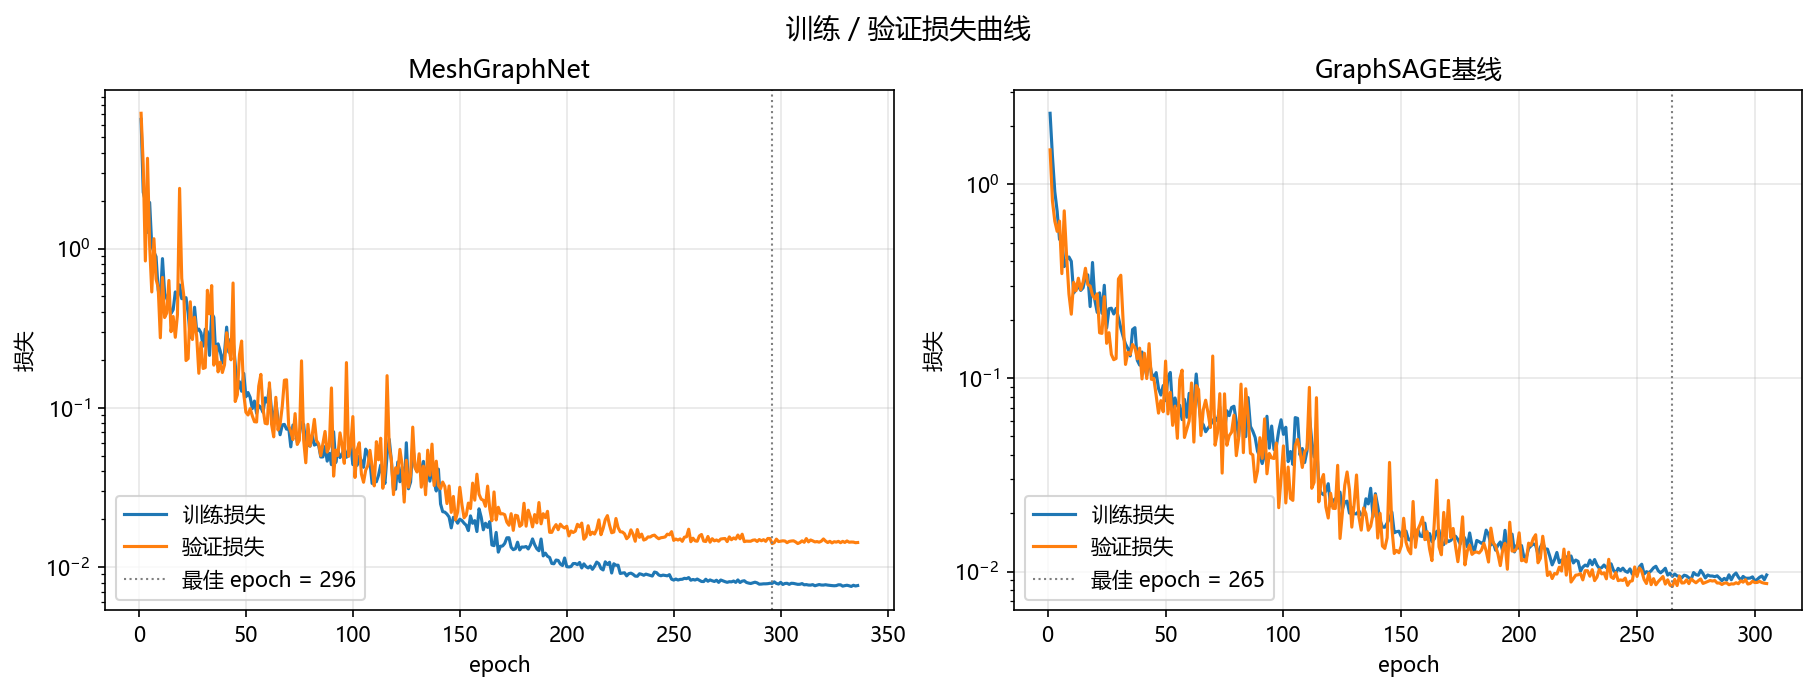
\includegraphics[width=0.98\textwidth]{loss_curves.png}
  \caption{MeshGraphNet 与 GraphSAGE 基线的训练/验证损失曲线（对数纵轴）。
  虚线标出验证集最优 epoch。}
  \label{fig:loss}
\end{figure}


% =========================================================
\section{评估指标与实验结果}
% =========================================================

评估在测试集 30 个样本上进行，硬件为 NVIDIA GeForce RTX 3060。指标定义：
\begin{itemize}[leftmargin=1.5em]
  \item \textbf{节点温度 MAE}：\(\frac{1}{N}\sum_i |\widehat{\Delta T}_i-\Delta T_i|\)；
  \item \textbf{相对 \(L_2\) 误差}：\(\|\widehat{\Delta T}-\Delta T\|_2 / \|\Delta T\|_2\)；
  \item \textbf{峰值温度绝对误差}：\(|\max\widehat{\Delta T}-\max\Delta T|\)；
  \item \textbf{\(R^2\)}：全测试集节点温升的决定系数；
  \item \textbf{耗时}：单样本推理、批量摊销推理与平均 FEM 求解时间。
\end{itemize}

\subsection{整体对比}
整体测试集结果见表~\ref{tab:overall}，柱状对比见图~\ref{fig:bars}。

\begin{table}[H]
\centering
\caption{测试集整体指标对比（实测）}
\label{tab:overall}
\resizebox{\textwidth}{!}{%
\begin{tabular}{lrrrrrrr}
\toprule
模型 & 参数量 & MAE [K] & 相对 \(L_2\) & 峰值误差 [K] & \(R^2\) & 单样本推理 [ms] & 批量摊销 [ms] \\
\midrule
MeshGraphNet & 979329 & 0.1095 & 0.2294 & 0.3562 & 0.9228 & 10.23 & 6.77 \\
GraphSAGE & 104321 & 0.1035 & 0.2231 & 0.3431 & 0.9270 & 2.08 & 0.46 \\
\bottomrule
\end{tabular}}
\end{table}

\begin{table}[H]
\centering
\caption{相对 FEM 的加速比（平均 FEM \(\approx 8.50\,\mathrm{ms}\)）}
\label{tab:speed}
\begin{tabular}{lccc}
\toprule
模型 & 单样本加速比 & 批量加速比 & 说明 \\
\midrule
MeshGraphNet & \(0.83\times\) & \(1.25\times\) & 小网格下 FEM 本身很快 \\
GraphSAGE & \(4.09\times\) & \(\mathbf{18.5\times}\) & 批量多工况扫描更有优势 \\
\bottomrule
\end{tabular}
\end{table}

\begin{figure}[H]
  \centering
  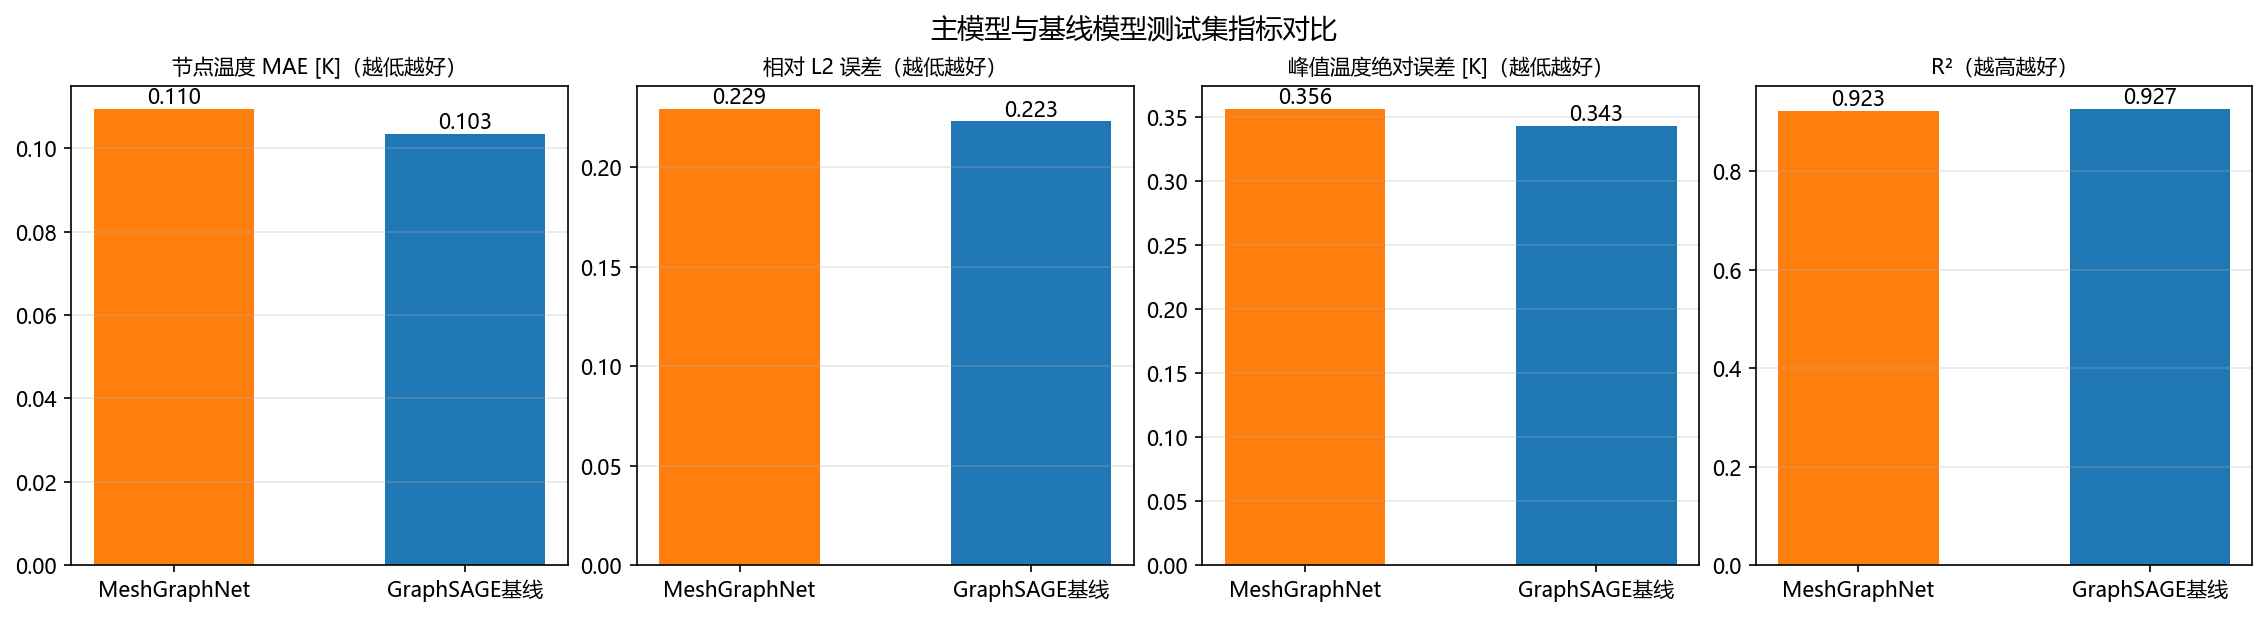
\includegraphics[width=0.98\textwidth]{metrics_bar.png}
  \caption{主模型与基线模型测试集指标柱状图对比。}
  \label{fig:bars}
\end{figure}

\textbf{解读：}
\begin{itemize}[leftmargin=1.5em]
  \item 在引入全局工况特征后，两模型整体精度接近，\(R^2>0.92\)；
  \item 本例网格仅约 2257 节点，稀疏直接法 FEM 本身极快，单样本 GNN 相对 FEM
  的加速有限；\textbf{批量多工况}下 GraphSAGE 可达约 \(18\times\)；
  \item 网格规模增大（如 \(10^5+\) 节点）时，FEM 成本上升更快，代理模型加速比通常更显著。
\end{itemize}

\subsection{分布内 / 分布外分拆}
表~\ref{tab:ood-mgn} 与表~\ref{tab:ood-base} 给出分工况指标。

\begin{table}[H]
\centering
\caption{MeshGraphNet：分布内 / OOD 分拆}
\label{tab:ood-mgn}
\begin{tabular}{lcccc}
\toprule
工况类型 & 样本数 & MAE [K] & 相对 \(L_2\) & 峰值误差 [K] \\
\midrule
分布内 (id) & 20 & 0.0389 & 0.0736 & 0.0807 \\
OOD 高功率 & 4 & 0.1867 & 0.1694 & 0.4634 \\
OOD 差 TIM & 3 & 0.2074 & 0.3844 & 0.9186 \\
OOD 差对流 & 3 & 0.3798 & 0.4422 & 1.4873 \\
\bottomrule
\end{tabular}
\end{table}

\begin{table}[H]
\centering
\caption{GraphSAGE 基线：分布内 / OOD 分拆}
\label{tab:ood-base}
\begin{tabular}{lcccc}
\toprule
工况类型 & 样本数 & MAE [K] & 相对 \(L_2\) & 峰值误差 [K] \\
\midrule
分布内 (id) & 20 & 0.0308 & 0.0627 & 0.0829 \\
OOD 高功率 & 4 & 0.1166 & 0.0860 & 0.1642 \\
OOD 差 TIM & 3 & 0.2156 & 0.3784 & 0.7643 \\
OOD 差对流 & 3 & 0.4589 & 0.6504 & 1.8947 \\
\bottomrule
\end{tabular}
\end{table}

分布内 MAE 约 \(0.03\sim 0.04\,\mathrm{K}\)，精度很高；OOD（尤其差对流）误差明显增大，
说明外推仍有挑战，同时也证明测试集确实包含训练集未见工况组合。

\subsection{峰值温度散点图}
图~\ref{fig:peak} 给出测试样本峰值温升真值--预测对比；红色三角为 OOD 样本。

\begin{figure}[H]
  \centering
  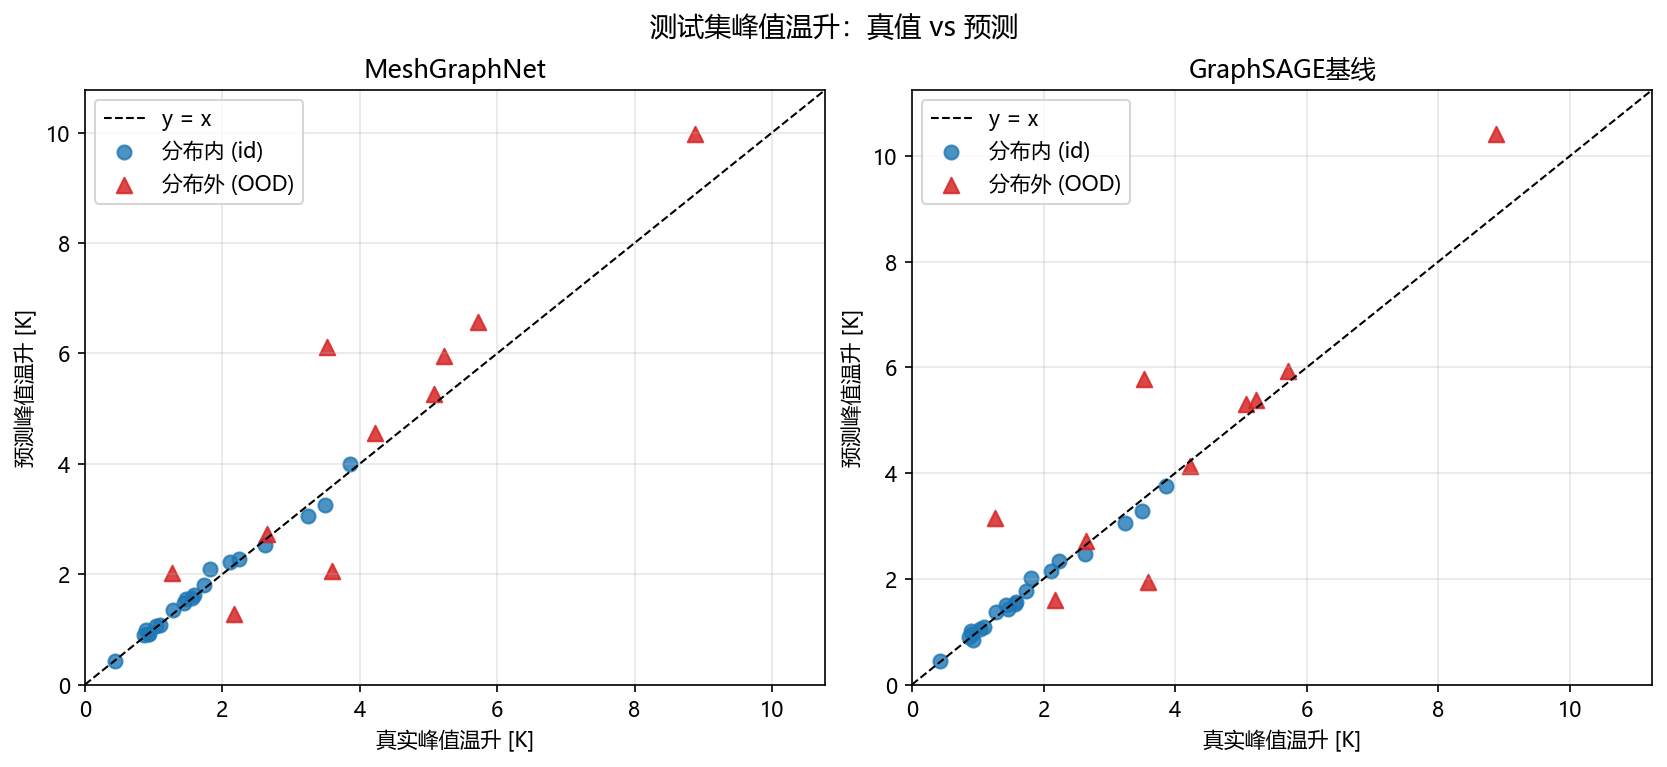
\includegraphics[width=0.95\textwidth]{peak_scatter.png}
  \caption{测试集峰值温升：真值 vs 预测。蓝色为分布内，红色三角为分布外。}
  \label{fig:peak}
\end{figure}


% =========================================================
\section{温度场可视化}
% =========================================================

对自动挑选的代表性测试样本，绘制真实温升场、预测温升场与误差场三联图。
图~\ref{fig:trip-mgn} 与图~\ref{fig:trip-base} 分别展示 MeshGraphNet 与基线结果
（含分布内与 OOD 样本）。

\begin{figure}[H]
  \centering
  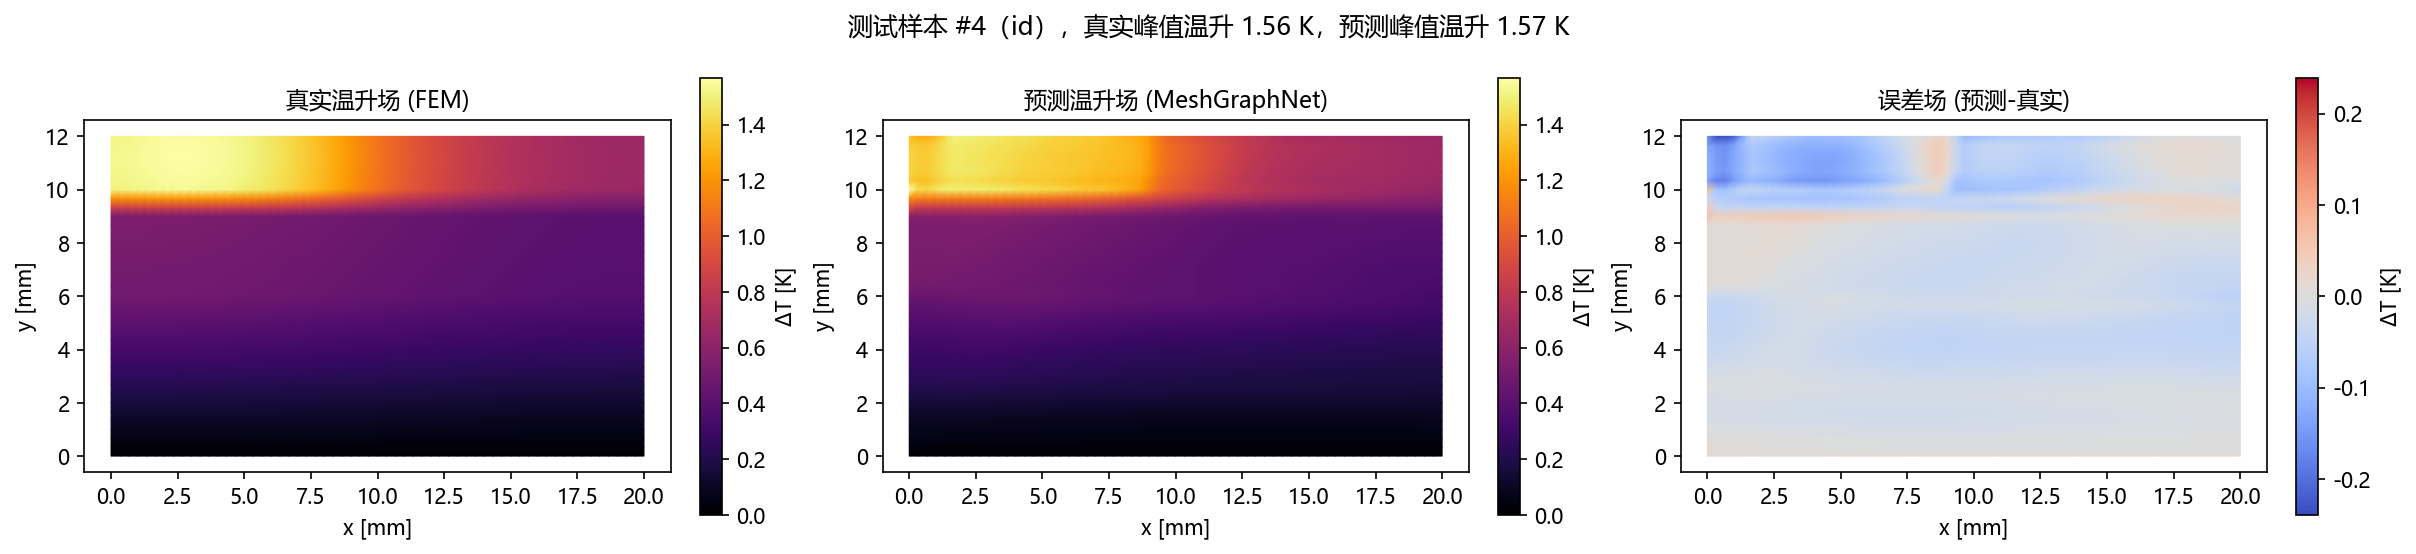
\includegraphics[width=0.98\textwidth]{field_triptych_meshgraphnet_sample4.png}\\[0.4em]
  {\small (a) 样本 4}\\[0.8em]
  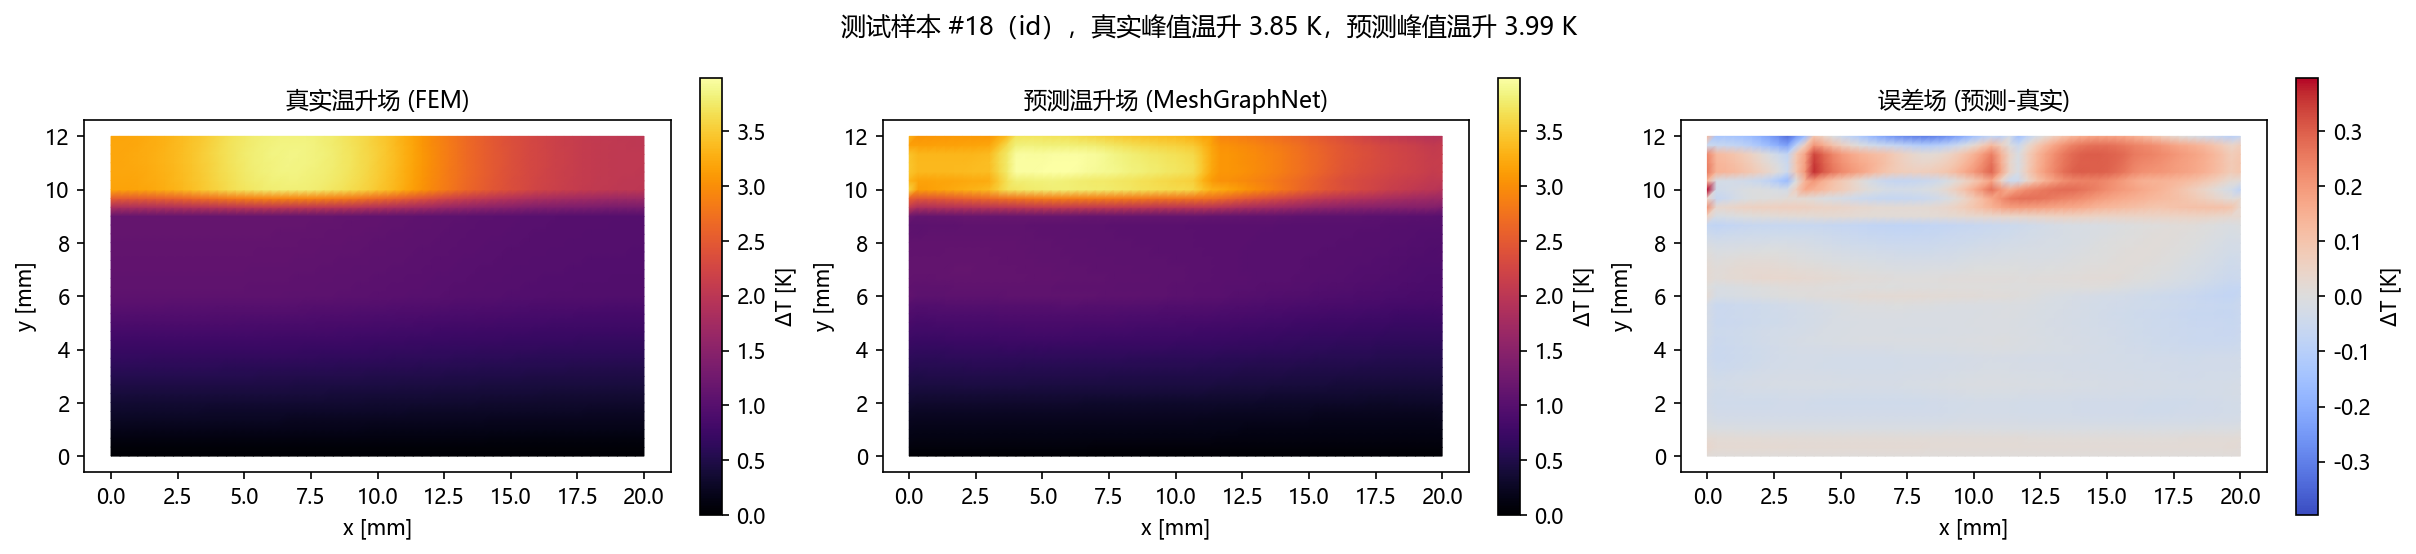
\includegraphics[width=0.98\textwidth]{field_triptych_meshgraphnet_sample18.png}\\[0.4em]
  {\small (b) 样本 18}\\[0.8em]
  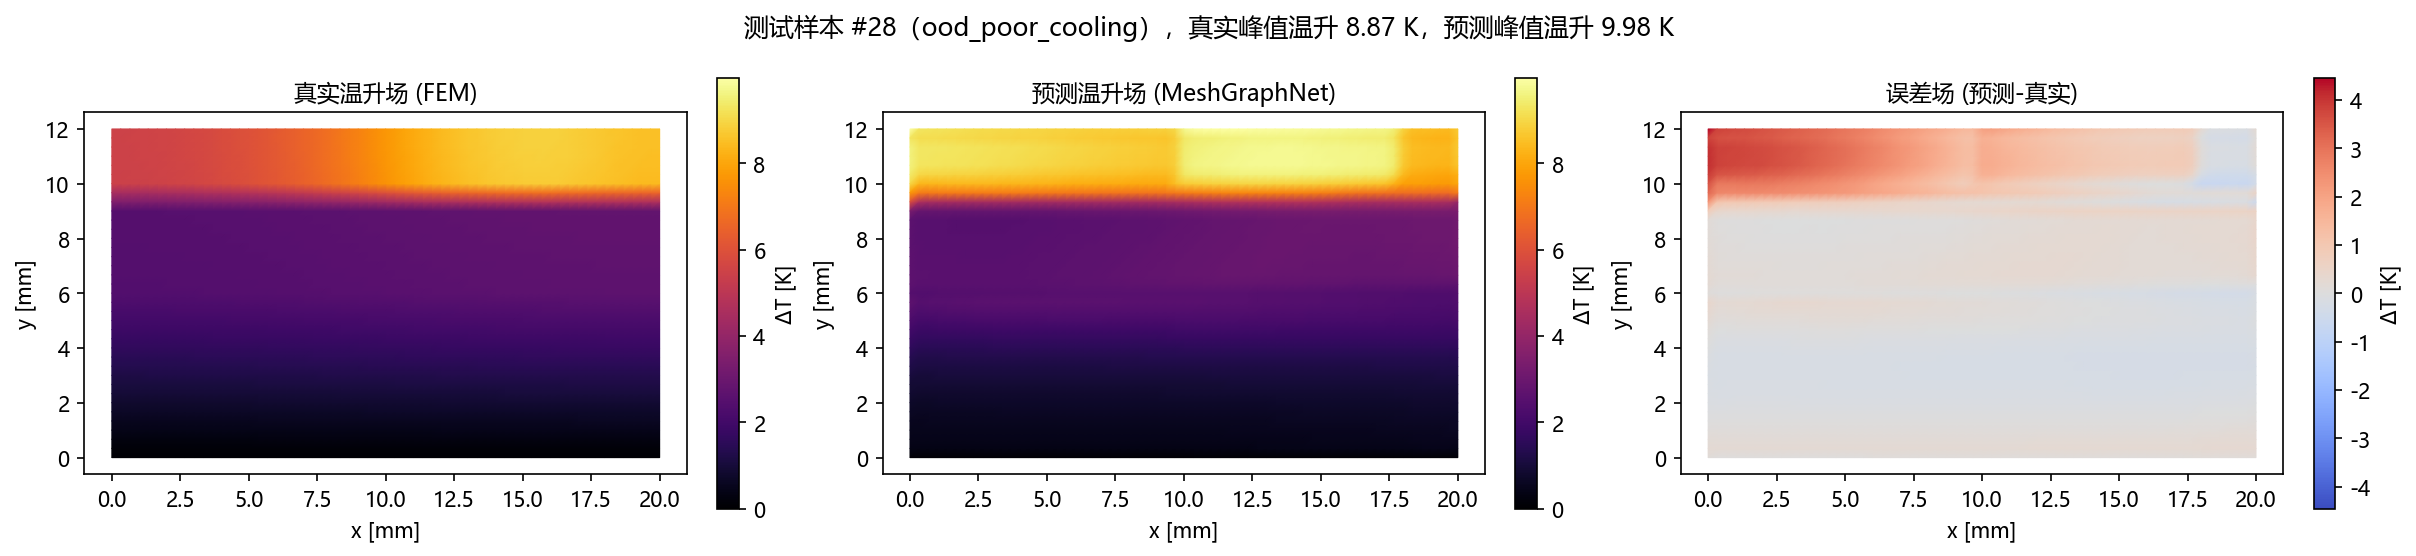
\includegraphics[width=0.98\textwidth]{field_triptych_meshgraphnet_sample28.png}\\[0.4em]
  {\small (c) 样本 28（含较高温升/OOD 倾向样本）}
  \caption{MeshGraphNet：真实温度场、预测温度场与误差场三联图。}
  \label{fig:trip-mgn}
\end{figure}

\begin{figure}[H]
  \centering
  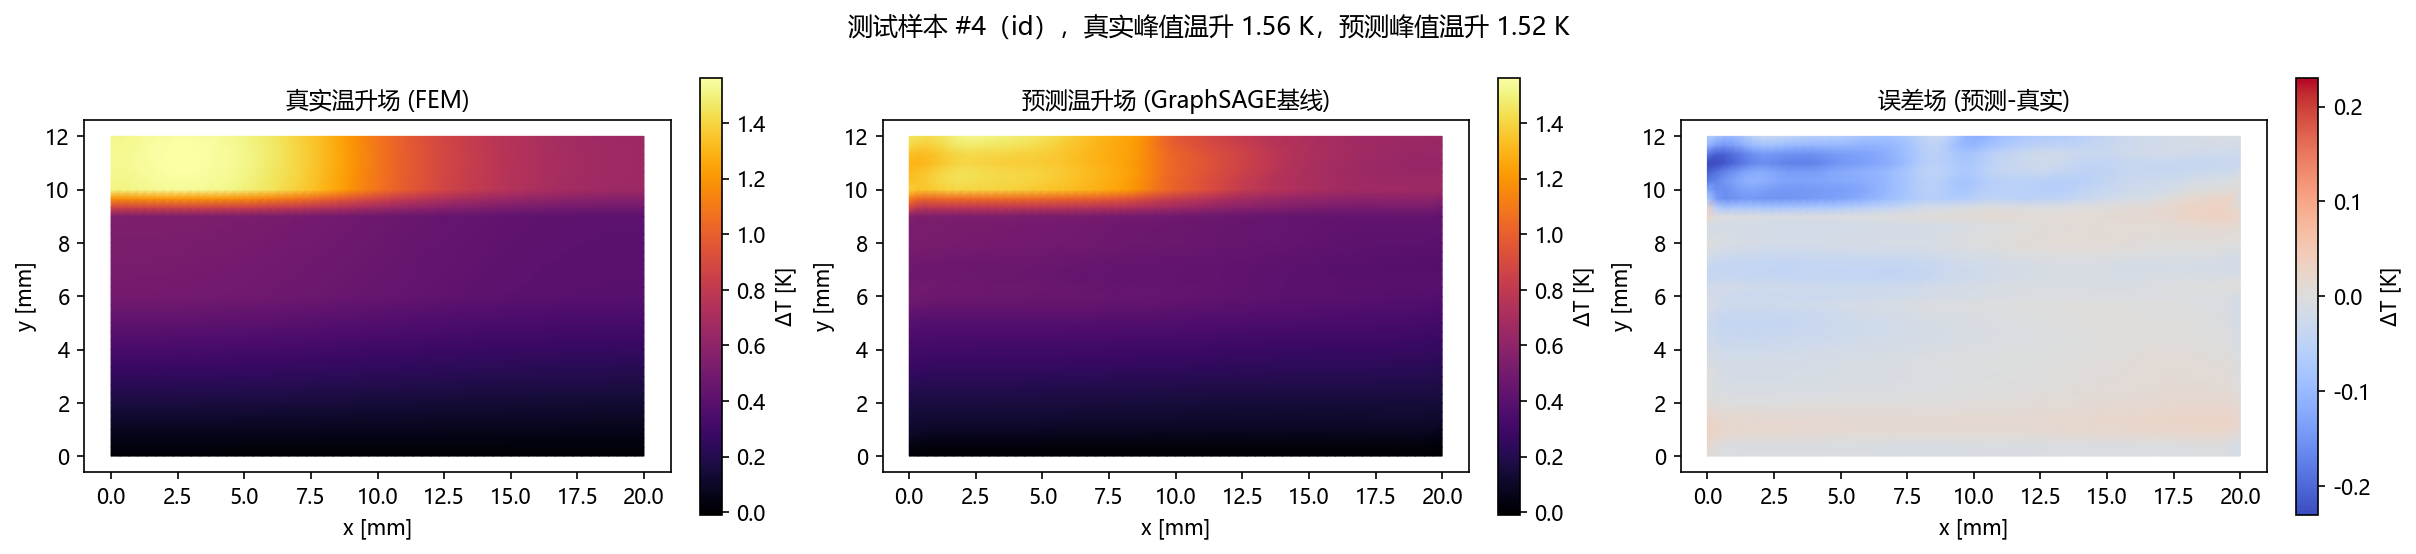
\includegraphics[width=0.98\textwidth]{field_triptych_baseline_sample4.png}\\[0.4em]
  {\small (a) 样本 4}\\[0.8em]
  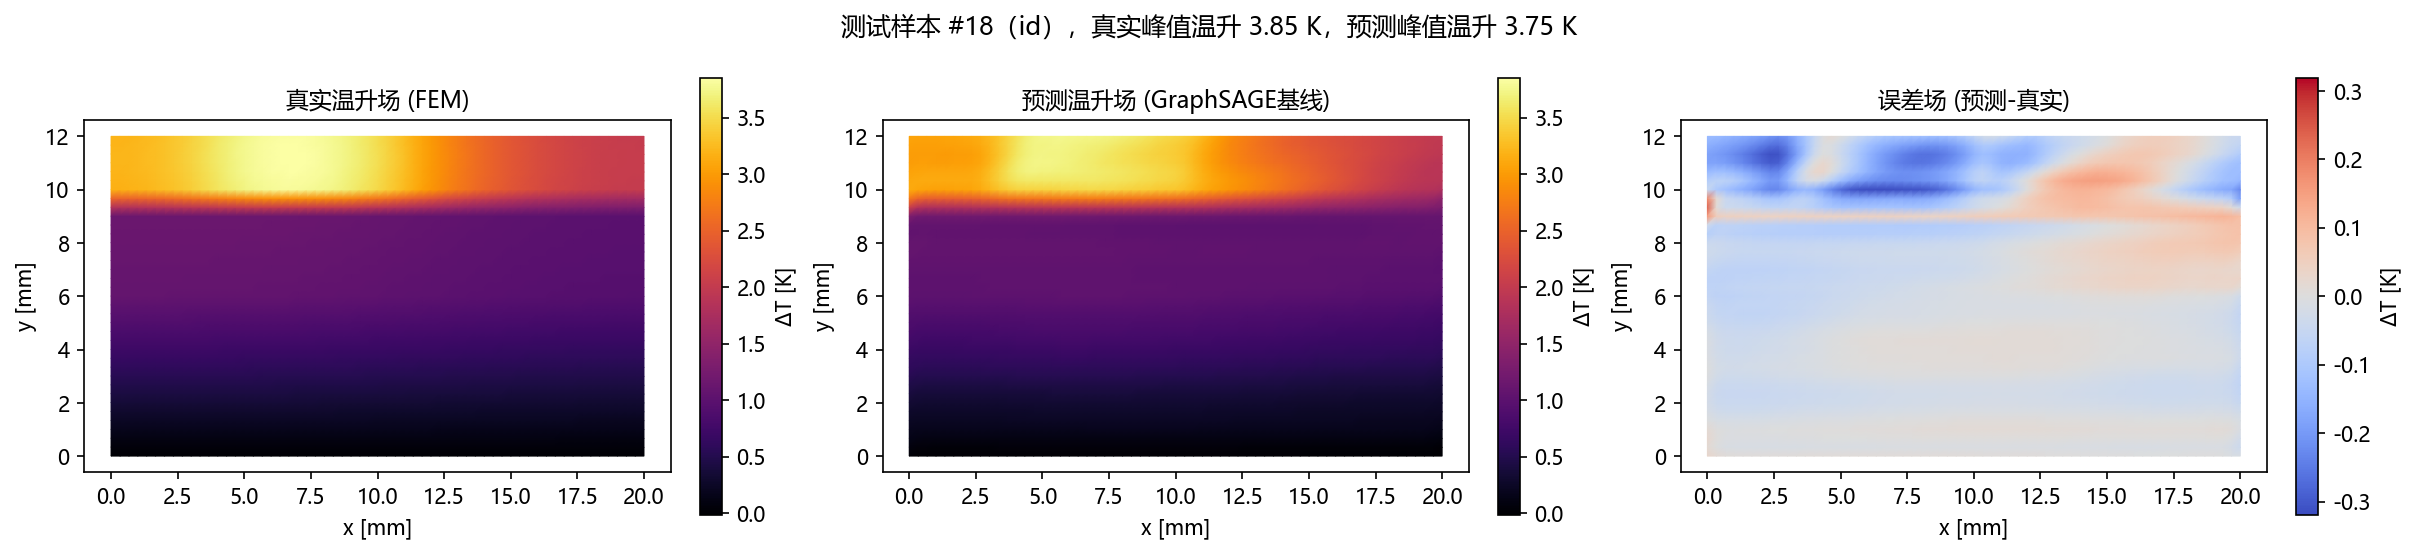
\includegraphics[width=0.98\textwidth]{field_triptych_baseline_sample18.png}\\[0.4em]
  {\small (b) 样本 18}\\[0.8em]
  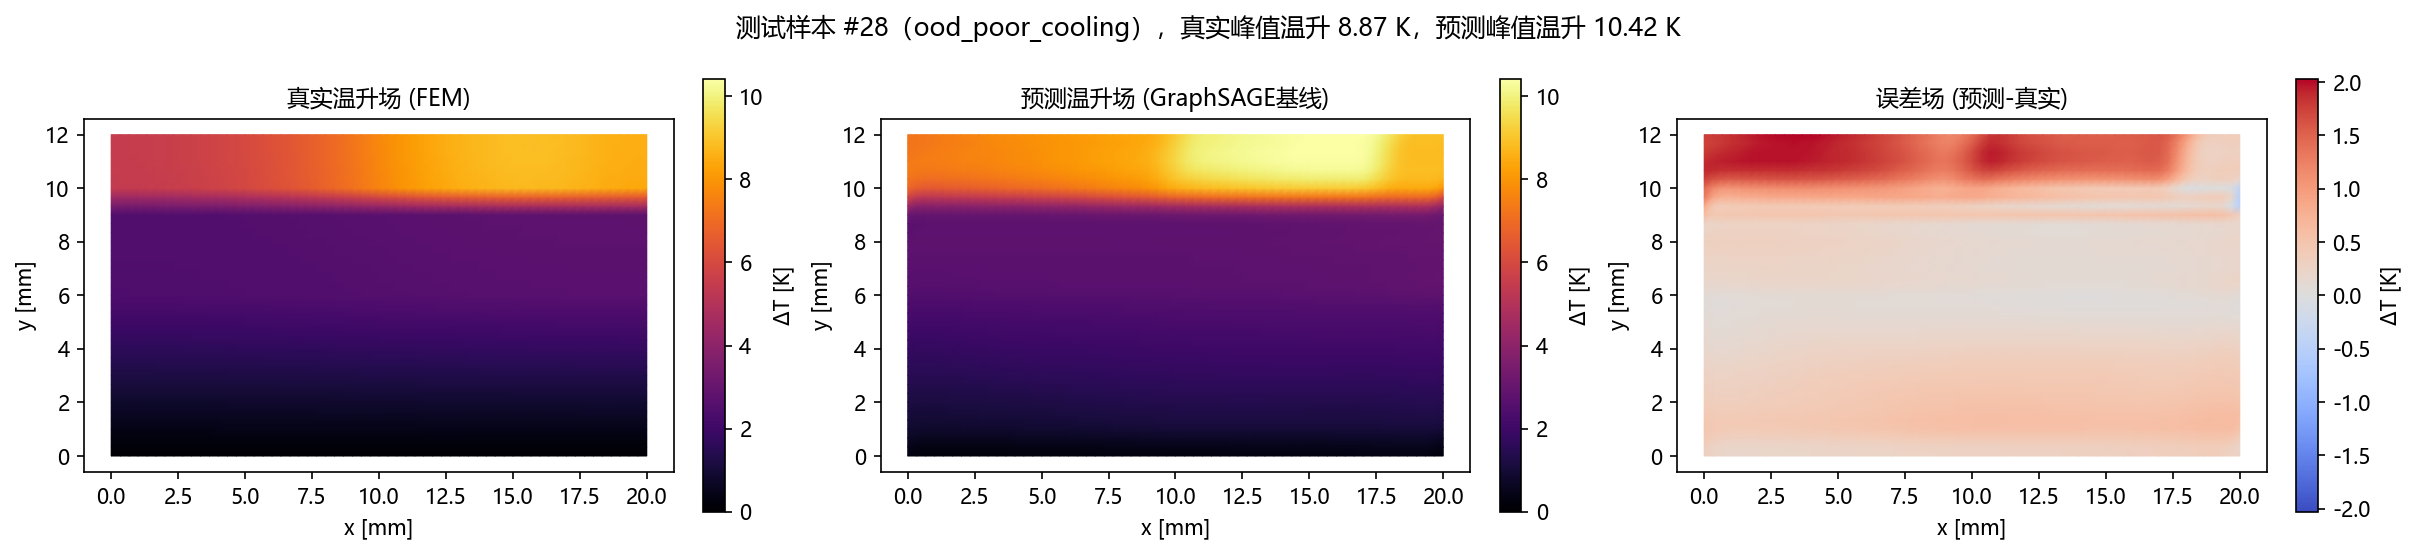
\includegraphics[width=0.98\textwidth]{field_triptych_baseline_sample28.png}\\[0.4em]
  {\small (c) 样本 28}
  \caption{GraphSAGE 基线：真实温度场、预测温度场与误差场三联图。}
  \label{fig:trip-base}
\end{figure}

从场图可见：分布内样本的热点位置与温升形态可被较好重建；误差主要集中在材料界面与
热点边缘等高梯度区域；OOD 样本的峰值误差相对更大。


% =========================================================
\section{复现实验步骤}
% =========================================================

\begin{lstlisting}
pip install -r requirements.txt

# 1. 生成 FEM 数据集（约 360 次求解）
python src/generate_dataset.py --config configs/data_config.yaml --out_dir data/raw

# 2. 网格 -> 图数据
python src/graph_dataset.py --raw_dir data/raw --out_dir data/processed

# 3. 训练
python src/train.py --model meshgraphnet
python src/train.py --model baseline

# 4. 评估
python src/evaluate.py

# 5. 可视化
python src/visualize.py

# 6. 单元测试
python -m pytest tests -q

# 7. 编译本说明文档（需 TeX Live / XeLaTeX）
cd docs
xelatex -interaction=nonstopmode report.tex
xelatex -interaction=nonstopmode report.tex
\end{lstlisting}

关键配置：
\begin{itemize}[leftmargin=1.5em]
  \item \texttt{configs/data\_config.yaml}：几何、材料/工况采样范围、OOD 设置、数据划分；
  \item \texttt{configs/train\_config.yaml}：模型超参数、损失类型、早停与学习率策略。
\end{itemize}


% =========================================================
\section{局限性与后续扩展}
% =========================================================

\subsection{当前局限性}
\begin{enumerate}[leftmargin=1.5em]
  \item 固定网格与固定几何，未验证跨网格/跨几何泛化；
  \item 二维简化，未建模三维热扩散；
  \item 线性稳态，无温度相关材料、辐射或接触热阻；
  \item 样本量适中（360），更大规模数据可进一步提升 OOD 外推；
  \item 小网格下相对 FEM 的单样本加速比有限。
\end{enumerate}

\subsection{从稳态扩展到瞬态}
\begin{enumerate}[leftmargin=1.5em]
  \item \textbf{数据端}：增加热容项 \(\rho c\,\partial T/\partial t\)，用隐式时间积分生成温度序列；
  \item \textbf{模型端}：改为自回归时间步进
  \(T(t+\Delta t)=T(t)+\mathrm{GNN}\big(T(t),\text{条件}\big)\)；
  \item \textbf{训练技巧}：输入噪声注入抑制 rollout drift，评估长时间稳定性；
  \item \textbf{应用}：支持时变功耗 \(q(t)\)，实现瞬态热响应预测。
\end{enumerate}


% =========================================================
\section{结论}
% =========================================================

本项目完成了从 FEM 数据生成、图构建、MeshGraphNet / GraphSAGE 训练、测试评估到可视化
的完整闭环。在分布内工况下，节点温升 MAE 可达约 \(0.03\sim 0.04\,\mathrm{K}\)，
整体 \(R^2\approx 0.92\sim 0.93\)；在 OOD 工况下误差增大，尤其差对流条件更具挑战。
在当前小规模网格上，代理模型的优势更体现在\textbf{批量多工况推理}；扩大网格规模后，
相对 FEM 的加速潜力将进一步体现。该系统可作为芯片封装热分析与 AI4S 演示的可复现基线。


\appendix
\section{主要输出文件索引}
\begin{itemize}[leftmargin=1.5em]
  \item 权重：\path{outputs/checkpoints/meshgraphnet_best.pt}，
  \path{outputs/checkpoints/baseline_best.pt}
  \item 指标：\path{outputs/metrics/model_comparison.csv}，
  \path{outputs/metrics/*_eval_summary.json}
  \item 图片：\path{outputs/figures/*.png}
  \item 原始元数据：\path{data/raw/metadata.json}
\end{itemize}

\end{document}
